\chapter{Diseño e implementación} % Main chapter title

\label{Chapter3} % Change X to a consecutive number; for referencing this chapter elsewhere, use \ref{ChapterX}

\definecolor{mygreen}{rgb}{0,0.6,0}
\definecolor{mygray}{rgb}{0.5,0.5,0.5}
\definecolor{mymauve}{rgb}{0.58,0,0.82}

%%%%%%%%%%%%%%%%%%%%%%%%%%%%%%%%%%%%%%%%%%%%%%%%%%%%%%%%%%%%%%%%%%%%%%%%%%%%%
% parámetros para configurar el formato del código en los entornos lstlisting
%%%%%%%%%%%%%%%%%%%%%%%%%%%%%%%%%%%%%%%%%%%%%%%%%%%%%%%%%%%%%%%%%%%%%%%%%%%%%
\lstset{ %
  backgroundcolor=\color{white},   % choose the background color; you must add \usepackage{color} or \usepackage{xcolor}
  basicstyle=\footnotesize,        % the size of the fonts that are used for the code
  breakatwhitespace=false,         % sets if automatic breaks should only happen at whitespace
  breaklines=true,                 % sets automatic line breaking
  captionpos=b,                    % sets the caption-position to bottom
  commentstyle=\color{mygreen},    % comment style
  deletekeywords={...},            % if you want to delete keywords from the given language
  %escapeinside={\%*}{*)},          % if you want to add LaTeX within your code
  %extendedchars=true,              % lets you use non-ASCII characters; for 8-bits encodings only, does not work with UTF-8
  %frame=single,	                % adds a frame around the code
  keepspaces=true,                 % keeps spaces in text, useful for keeping indentation of code (possibly needs columns=flexible)
  keywordstyle=\color{blue},       % keyword style
  language=[ANSI]C,                % the language of the code
  %otherkeywords={*,...},           % if you want to add more keywords to the set
  numbers=left,                    % where to put the line-numbers; possible values are (none, left, right)
  numbersep=5pt,                   % how far the line-numbers are from the code
  numberstyle=\tiny\color{mygray}, % the style that is used for the line-numbers
  rulecolor=\color{black},         % if not set, the frame-color may be changed on line-breaks within not-black text (e.g. comments (green here))
  showspaces=false,                % show spaces everywhere adding particular underscores; it overrides 'showstringspaces'
  showstringspaces=false,          % underline spaces within strings only
  showtabs=false,                  % show tabs within strings adding particular underscores
  stepnumber=1,                    % the step between two line-numbers. If it's 1, each line will be numbered
  stringstyle=\color{mymauve},     % string literal style
  tabsize=2,	                   % sets default tabsize to 2 spaces
  title=\lstname,                  % show the filename of files included with \lstinputlisting; also try caption instead of title
  morecomment=[s]{/*}{*/}
}
En este capítulo se enumeran y desarrollan los aspectos considerados a la hora diseñar el robot. Se tuvieron en cuenta los alcances establecidos y las posibilidades económicas de solventar el proyecto.

%----------------------------------------------------------------------------------------
%	SECTION 1
%----------------------------------------------------------------------------------------


\section{Diseño de software}

Para la arquitectura del firmware se tuvo en cuenta un patrón de diseño de arquitectura de control ambiental \citep{arq}, ya que se trata de un patrón de control general que incluye procesos de sensor y actuador, y es el que más se acerca al modelo de comportamiento del robot. En respuesta a los cambios ambientales detectados por los sensores, se envían señales de control a los actuadores del sistema. En la figura \ref{fig:arq2} se muestra un esquema de la arquitectura utilizada.

\begin{figure}[h]
	\centering
	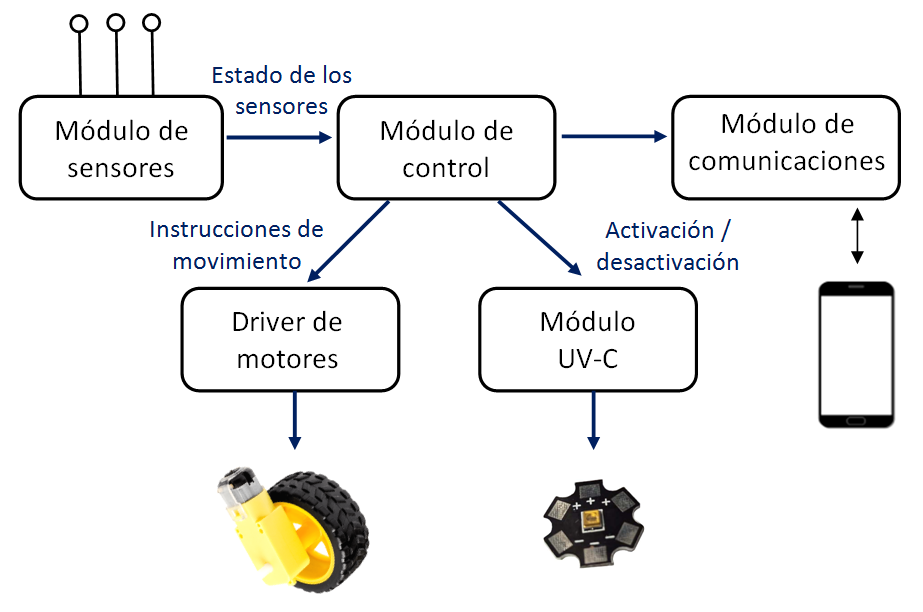
\includegraphics[width=13cm]{./Figures/arquitectura.PNG}
	\caption{Esquema de la arquitectura de firmware del robot.}
	\label{fig:arq2}
\end{figure}


\begin{itemize}
	\item Modulo de sensores del robot: inicializa y levanta datos de los distintos sensores. Elabora una estructura de datos con los estados de los sensores para ser utilizada por el Módulo principal de Control.
	\item Driver de motores. se encarga de inicializar y controlar la electrónica relacionada con los motores según las indicaciones recibidas desde el Módulo principal de Control.  
	\item Modulo UV-C: activa y desactiva el módulo UV, según indicación del módulo principal de control. Debe poder indicar si el módulo está funcionando o no, o si ha detectado algún inconveniente. 
	\item Modulo de comunicaciones: inicializa y establece comunicación con la aplicación externa. Verifica que se ha establecido el enlace.
	\item  Módulo principal de control: se encarga de inicializar los demás módulos y determinar el comportamiento general del dispositivo. Recibe datos de sensores desde el módulo de sensores y envía indicaciones de movimiento al módulo Control de motores, recibiendo realimentación del mismo. Activa y desactiva el módulo UV. Establece comunicación con la aplicación externa a través de módulo de comunicaciones.
\end{itemize}




\subsection{Estructura de capas}
El diseño del firmware se organizó como una estructura de capas, lo cual permite la separación de las partes que componen el sistema. 
La programación se realizó utilizando lenguaje C sobre el firmware de la EDU-CIAA versión 3 como capa de abstracción de hardware y se utilizaron módulos de software de la biblioteca sAPI para acceder de manera simple a los diferentes periféricos.
Se modularizó el firmware en archivos, de modo de mantener en un mismo módulo de software las instrucciones relacionadas con cada periférico y que puedan utilizarse (y reutilizarse) en forma ordenada. Se usó una máquina de estados finitos como rutina principal para el comportamiento autónomo del robot, en función reactiva a la información obtenida por los sensores.
En la figura \ref{fig:capas} se muestra el esquema de capas utilizado.

\begin{figure}[h]
	\centering
	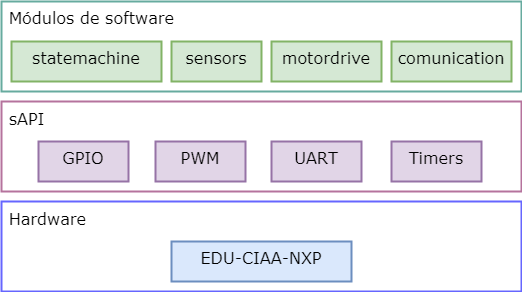
\includegraphics[width=11cm]{./Figures/capas.png}
	\caption{Esquema de capas.}
	\label{fig:capas}
\end{figure}

\subsection{Módulos de software}


\subsubsection{Comunicaciones}

El módulo de software dedicado a las comunicaciones se encarga de:

\begin{itemize}
	\item Iniciar y configurar la UART.
	\item Establecer comunicación con la aplicación móvil.
	\item Recibir los mensajes de la aplicación y generar las acciones correspondientes (movimientos).
	\item Envíar a la aplicación las notificaciones de reconocimiento o error.
\end{itemize}

Para la comunicación serie entre dispositivos a través del periférico UART se utilizaron las funciones de la biblioteca sAPI.
Para la ejecución de las instrucciones de movimiento que se reciben de la aplicación móvil, el módulo de comunicaciones envía comandos codificados al módulo de control de motores, indicando la acción a realizar un un parámetro modificador,



\subsubsection{Máquina de estados finitos}

Las Máquinas de Estado Finitas (FSM, por su sigla en inglés) \citep{FSMbook} son utilizadas ampliamente como rutinas para reconocimiento de secuencias de datos, para interpretación de tramas de comunicación serie, y para el ordenamiento de tareas ante distintas condiciones medidas. Son básicamente estructuras de programa cuyo comportamiento está determinado por el estado en el que se encuentran y por variables (generalmente booleanas) de entrada, ofreciendo para cada caso una salida y un estado próximo, que puede tratarse del mismo estado en el que se encuentra.
Su uso es sencillo, implica un bajo consumo de procesamiento, y resulta flexible para el agregado de nuevas condiciones y estados. Sin embargo, cuando el número de entradas crece, su implementación y mantenimiento puede resultar complejo ya que su comportamiento se establece en el código fuente. En la figura \ref{fig:estados} se muestra un esquema de máquina de estados como el utilizado en el control del robot.

\begin{figure}[h]
	\centering
	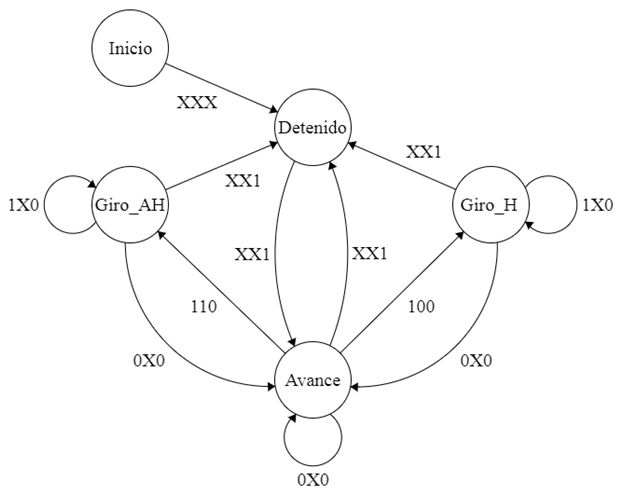
\includegraphics[width=12cm]{./Figures/estados.png}
	\caption{Esquema de máquina de estados como el utilizado en el control del robot.}
	\label{fig:estados}
\end{figure}


Los estados están asociados a las acciones que realiza el robot:
\begin{itemize}
	\item Estado detenido: el robot se encuentra detenido.
	\item Estado avance: el robot se encuentra avanzando hacia delante.
	\item Estado giro h: el robot se encuentra girando en sentido horario.
	\item Estado giro ah: el robot se encuentra girando en sentido antihorario.
\end{itemize}

Se utilizó un método en el que la máquina de estados se actualiza a partir de los datos registrados en  una estructura de datos de estados/entradas/salidas almacenada en un archivo header en la memoria del microcontrolador (librería MdE.h). Las variables de entrada son de tipo booleano y las acciones planteadas por la tabla corresponden a comportamientos puramente reactivos. La solución ha sido presentada en un trabajo de investigación anterior \citep{planilla}. En la la figura \ref{fig:flujo} se representa en forma de diagrama de flujo la secuencia de la máquina de estados cuyas acciones responden a las directivas tomadas desde la tabla de la librería MdE.h.


\begin{figure}[h]
	\centering
	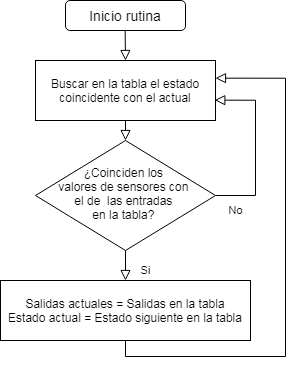
\includegraphics[width=7
	cm]{./Figures/flujo.png}
	\caption{Diagrama de flujo básico de la rutina de la máquina de estados.}
	\label{fig:flujo}
\end{figure}


La ventaja del método utilizado radica en el uso de una aplicación en una PC que permite generar el contenido del archivo header a partir de una hoja de cálculo en la que se pueden consignar las distintas acciones a partir de las combinaciones de estado actual y condiciones de entrada. 


En la planilla de configuración, es posible “enmascarar” condiciones que son indiferentes al comportamiento  usando el valor “X” (interpretado semánticamente como “indeterminado”), que luego es expandido por la aplicación intérprete de modo que finalmente en la estructura de datos de la FSM se consideren todas las condiciones como valores booleanos. 

La aplicación verifica que no se produzcan combinaciones redundantes o inválidas y se encarga de construir el archivo header con la estructura ordenada de datos para la actualización de la FSM, que luego puede ser transferido al microcontrolador del robot.
En la figura \ref{fig:MdE} se observa un ejemplo de configuración de la FSM con una tabla escrita en una planilla de cálculo.


\begin{figure}[h]
	\centering
	\includegraphics[width=\textwidth]{./Figures/MdE.PNG}
	\caption{Ejemplo de configuración de la FSM con una tabla escrita en una planilla de cálculo.}
	\label{fig:MdE}
\end{figure}



La FSM se implementa como rutina principal, tomando los datos de la tabla procesada y consignada en el archivo header, y partiendo siempre de un estado inicial. La rutina de la FSM utiliza pocos recursos de procesamiento, relevando las variables de entrada y el valor del estado actual, y localizando en la tabla la opción de salida y el estado al que debe pasar .
		
Este método reduce considerablemente el tamaño del código de la rutina de actualización de FSM, a la vez que facilita realizar cambios en el comportamiento del robot al cambiar solo los datos en la librería MdE.h. 
En el código \ref{code:mde} se observa el listado de los valores ordenados y expandidos a partir de la tabla de la figura \ref{fig:MdE}.
		
\begin{lstlisting}[caption= Ejemplo de estructura de datos almacenada en MdE.h , label=code:mde]
// **************  TABLA  *********************
unsigned char Planilla [60][6] = 
{
    {0,0,16,1,100,1},
    {0,0,17,1,100,1},
    {0,0,18,1,100,1},
    {0,0,19,1,100,1},
    {0,0,20,1,100,1},
    {0,0,21,1,100,1},
    {0,0,22,1,100,1},
    {0,0,23,1,100,1},
    {0,0,24,1,100,1},
    {0,0,25,1,100,1},
    {0,0,26,1,100,1},
    {0,0,27,1,100,1},
    {0,0,28,1,100,1},
    {0,0,29,1,100,1},
    {0,0,30,1,100,1},
    {0,0,31,1,100,1},
    {1,0,0,1,100,1},
    {1,0,0,3,120,1},
    {1,0,1,3,120,1},
    {1,0,1,3,90,1},
    {1,0,2,3,120,1},
    {1,0,3,2,90,1},
    {1,0,3,3,120,1},
    {1,0,4,3,120,1},
    {1,0,5,3,120,1},
    {1,0,6,3,120,1},
    {1,0,7,3,120,1},
    {1,0,8,2,120,1},
    {1,0,8,3,120,1},
    {1,0,9,2,120,1},
    {1,0,9,3,120,1},
    {1,0,10,2,120,1},
    {1,0,10,3,120,1},
    {1,0,11,2,120,1},
    {1,0,11,3,120,1},
    {1,0,12,2,120,1},
    {1,0,12,3,120,1},
    {1,0,13,2,120,1},
    {1,0,13,3,120,1},
    {1,0,14,3,120,1},
    {1,0,14,2,120,1},
    {1,0,15,2,120,1},
    {1,0,15,3,120,1},
    {1,0,16,1,0,0},
    {1,0,17,1,0,0},
    {1,0,18,1,0,0},
    {1,0,19,1,0,0},
    {1,0,20,1,0,0},
    {1,0,21,1,0,0},
    {1,0,22,1,0,0},
    {1,0,23,1,0,0},
    {1,0,24,1,0,0},
    {1,0,25,1,0,0},
    {1,0,26,1,0,0},
    {1,0,27,1,0,0},
    {1,0,28,1,0,0},
    {1,0,29,1,0,0},
    {1,0,30,1,0,0},
    {1,0,31,1,0,0},
    {255,0,0,0,0,0}
};
\end{lstlisting}		
		
		
		\subsubsection{Sensores}

El módulo de software dedicado a loa sensores (sensors.c) se encarga de inicializar las variables relacionadas con los sensores, y realizar la lectura de cada uno de ellos. Para facilitar el tratamiento de la información de los sensores se representan sus estados con valores booleanos en un única variable que se utiliza como entrada en la máquina de estados. 
	
		
		\subsubsection{Motores}

El módulo de software dedicado al control de los motores se encarga de controlar el estado de marcha de los dos motores de corriente continua. 
Se encarga de inicializar la función PWM de la capa de abstracción (sAPI) y setear las dos salidas de PWM  para determinar la velocidad de giro de cada motor, además controlar las líneas GPIO correspondientes para el accionamiento del puente H del módulo L298.
El módulo de motores recibe de la máquina de estados la indicación de qué acción debe realizar cada motor en cada momento, en concordancia con los estados (Avanzar, girar o detenerse). Las acciones se codificaron por medio de un número identificador de tarea(ID) y un parámetro modificador, que da mayor detalle sobre la acción a realizar.
Esta codificación de acciones se realizó con el fin de simplificar el uso de la tabla de configuración de la máquina de estado, de modo que las acciones a realizar queden unívocamente identificadas con valores numéricos.
Por ejemplo a la acción avanzar le corresponde el ID número 1, con lo que se activarán los dos motores en forma simultánea y en la misma dirección,  mientras que el valor que lo acompaña (entre 0 y 255) determina el valor de PWM que se aplicará a los motores.



\subsection{Aplicación móvil}

La aplicación móvil de control externo fue desarrollada con el entorno MIT App Inventor. 
El diseño incluye un boton de selección de dispositivo, tres botones de dirección (hacia adelante, giro a la derecha y giro a la izquierda). dos botones para el accionamiento del módulo UV-C y un área de mensajes para indicación de reconocimiento o error. 

El programa de la aplicación se encarga de la inicalización de la comunicación con el robot y de enviar la información correspondiente a cada acción a realizar.
En la figura \ref{fig:mitapp} se muestra el formato de la programación en bloques de la aplicación.

\begin{figure}[h]
	\centering
	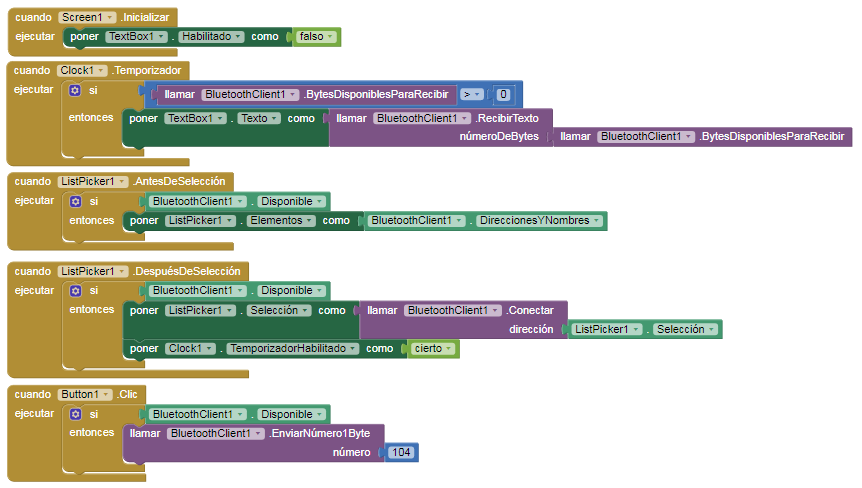
\includegraphics[width=14cm]{./Figures/mitapp.PNG}
	\caption{Programación en bloques usando App Inventor Blocks Editor.}
	\label{fig:mitapp}
\end{figure}
%
%\pagebreak

En la figura \ref{fig:pantalla} se muestra cómo queda configurada la pantalla de la aplicación móvil implementada con MIT App Inventor.

\begin{figure}[h]
	\centering
	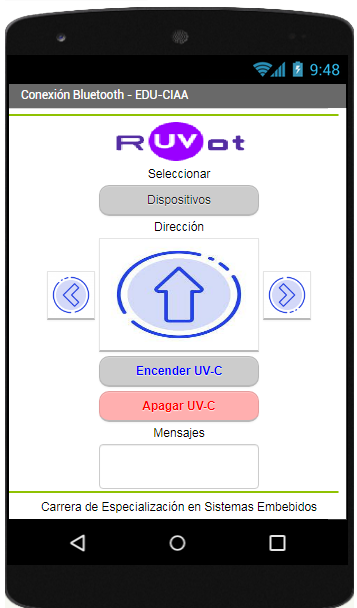
\includegraphics[width=5cm]{./Figures/pantallaruvot2.PNG}
	\caption{Imagen de la pantalla de la aplicación móvil implementada con MIT App inventor.}
	\label{fig:pantalla}
\end{figure}


\pagebreak



%----------------------------------------------------------------------------------------
%	SECTION 3
%----------------------------------------------------------------------------------------



\section{Diseño mecánico}

En esta sección se presenta la conformación del prototipo desde un punto de vista mecánico. Se describe el diseño del chasis y la carcasa del robot,  la estructura sobre la que se monta la totalidad de los componentes, las características de los motores y demás partes constitutivas.



\subsection{Diseño del chasis}
Se optó por una configuración de tracción de tipo diferencial \citep{traccion} que permite al robot girar sobre su propio eje, moverse en espacios interiores y evitar obstáculos sin quedar atascado. Se usan dos ruedas controladas individualmente junto con una rueda giratoria (caster wheel en inglés) como tercer punto de apoyo.
Se construyó una base en acrílico para montar los motores y colocar encima las placas electrónicas de control y accionamiento del robot. En la figura \ref{fig:base} se muestra la base y la distribución física de los motores. 

\begin{figure}[h]
	\centering
	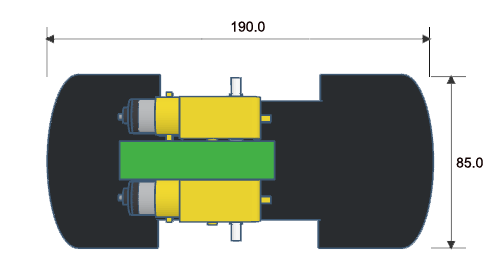
\includegraphics[width=11cm]{./Figures/base.png}
	\caption{Base y distribución de los motores.}
	\label{fig:base}
\end{figure}

Las dimensiones de esta base se determinaron en función del tamaño de los motores y de la placa principal de procesamiento. En la figura \ref{fig:baseeduciaa} se muestra la base en relación con la placa de procesamiento, ruedas y baterías. 

\begin{figure}[h]
	\centering
	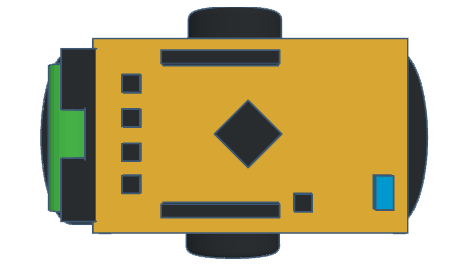
\includegraphics[width=10cm]{./Figures/baseeduciaa.png}
	\caption{Ubicación de la placa EDU-CIAA, ruedas y baterías en la base.}
	\label{fig:baseeduciaa}
\end{figure}

Para facilitar el movimiento de la plataforma robot, en configuración diferencial, se incluyó un tercer punto de apoyo o  rueda giratoria que mantiene al robot horizontal durante su movimiento. La pieza se compone de un soporte impreso en 3D, y una bola que se mueve libremente dentro del soporte. En la figura \ref{fig:ballcater} se observa la imagen 3D de la pieza impresa.


\begin{figure}[h]
	\centering
	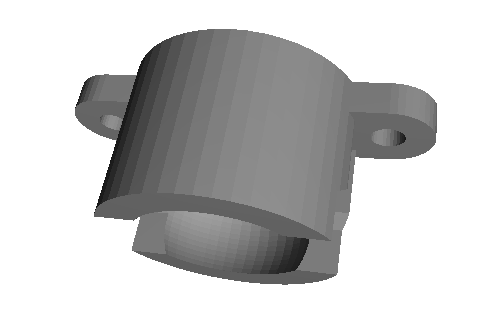
\includegraphics[width=4cm]{./Figures/ballcater.PNG}
	\caption{Imagen 3D de la pieza para el tercer punto de apoyo del robot.}
	\label{fig:ballcater}
\end{figure}


\subsection{Diseño de la carcasa del robot}

El chasis se completa con una base circular sobre la que se integran los sensores y el resto de la carcasa. Esta forma responde a la necesidad de evitar que el robot quede atorado entre obstáculos (como pueden ser patas de mesas o sillas). La base circular sumada a la tracción diferencial permite al robot salir de cualquier encrucijada por el mismo camino por el que accedió, ya que puede rotar sobre sí mismo y no presenta irregularidades que puedan trabarse. En la figura \ref{fig:base2} se muestra la integración de la base inicial con el chasis circular. 

\begin{figure}[h]
	\centering
	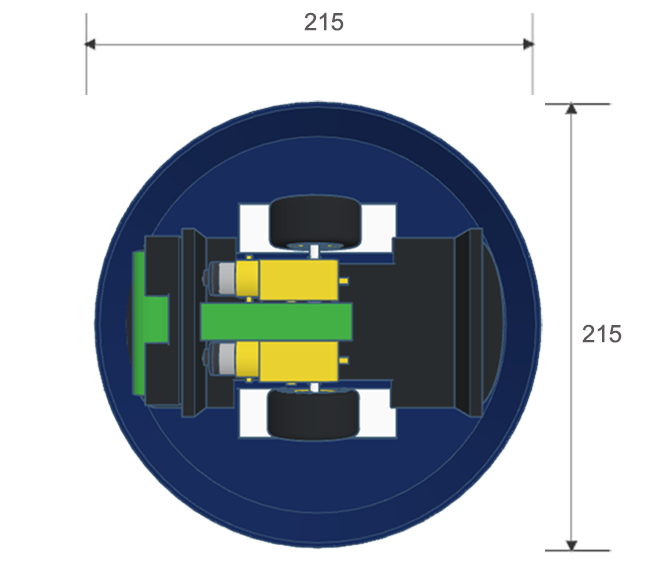
\includegraphics[width=12cm]{./Figures/base2.png}
	\caption{Base circular.}
	\label{fig:base2}
\end{figure}

En la figura \ref{fig:basearmada} se muestra una vista 3D  de la base y los componentes principales: motores y sus drivers, ruedas, baterías y placas de control.

\begin{figure}[h]
	\centering
	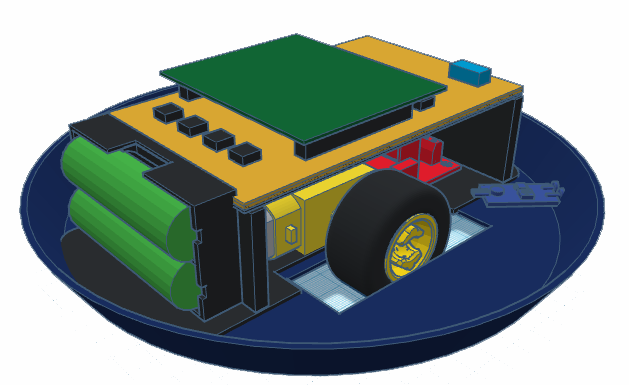
\includegraphics[width=12cm]{./Figures/basearmada.png}
	\caption{Modelo 3D de la base y componentes.}
	\label{fig:basearmada}
\end{figure}


En la figura \ref{fig:rUVot13xsintapa} se muestra una vista 3D de la base completa con la tapa y el sensor PIR en la parte superior.

\begin{figure}[h]
	\centering
	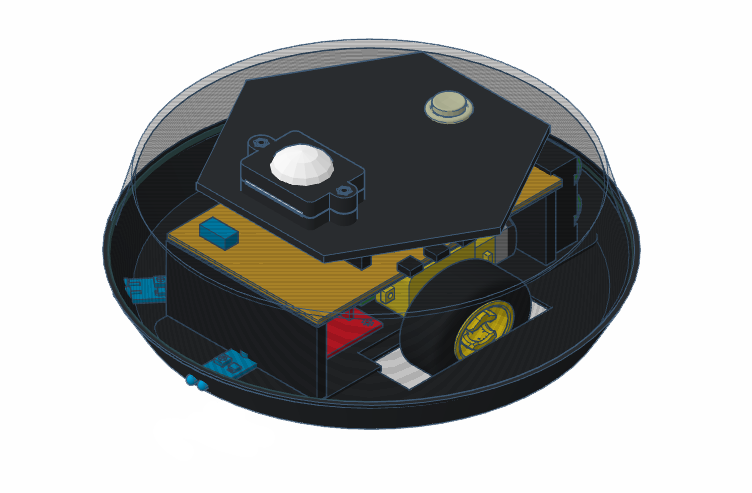
\includegraphics[width=13cm]{./Figures/rUVot13xsintapa.PNG}
	\caption{Imagen 3D de la base completa con la tapa y el sensor PIR.}
	\label{fig:rUVot13xsintapa}
\end{figure}

Se imprimió en 3D una carcasa para el módulo PIR, de modo que quede expuesta la parte que permite el sensado a la vez que se protege la placa electrónica y se facilita su montaje en la parte superior del robot. En la figura \ref{fig:pircase} se muestra se observa la imagen 3D de la carcasa para el módulo PIR.


\begin{figure}[h]
	\centering
	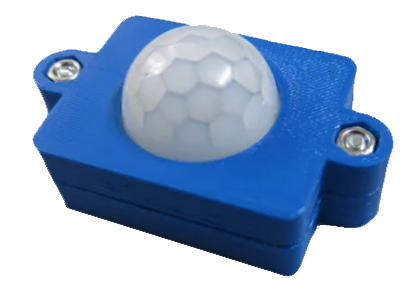
\includegraphics[width=5cm]{./Figures/pircase.PNG}
	\caption{Imagen 3D de la carcasa para el módulo PIR.}
	\label{fig:pircase}
\end{figure}

\pagebreak




%\begin{figure}[h]
%	\centering
%	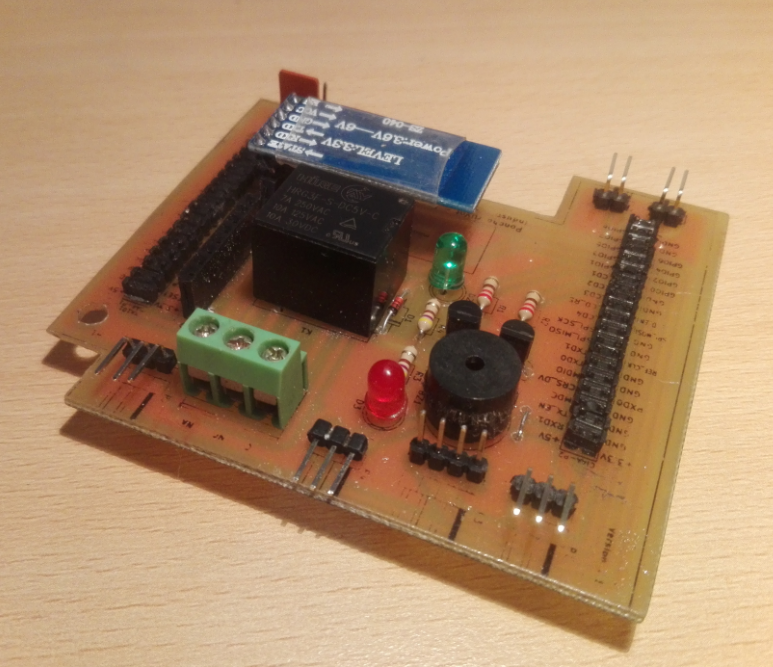
\includegraphics[width=11cm]{./Figures/placafoto2.png}
%	\caption{Fotografía de la placa desarrollada.}
%	\label{fig:placafoto2}
%\end{figure}



%presenta el circuito esquemático del poncho donde se puede observar el conexionado eléctrico.

%\begin{figure}[h]
%	\centering
%	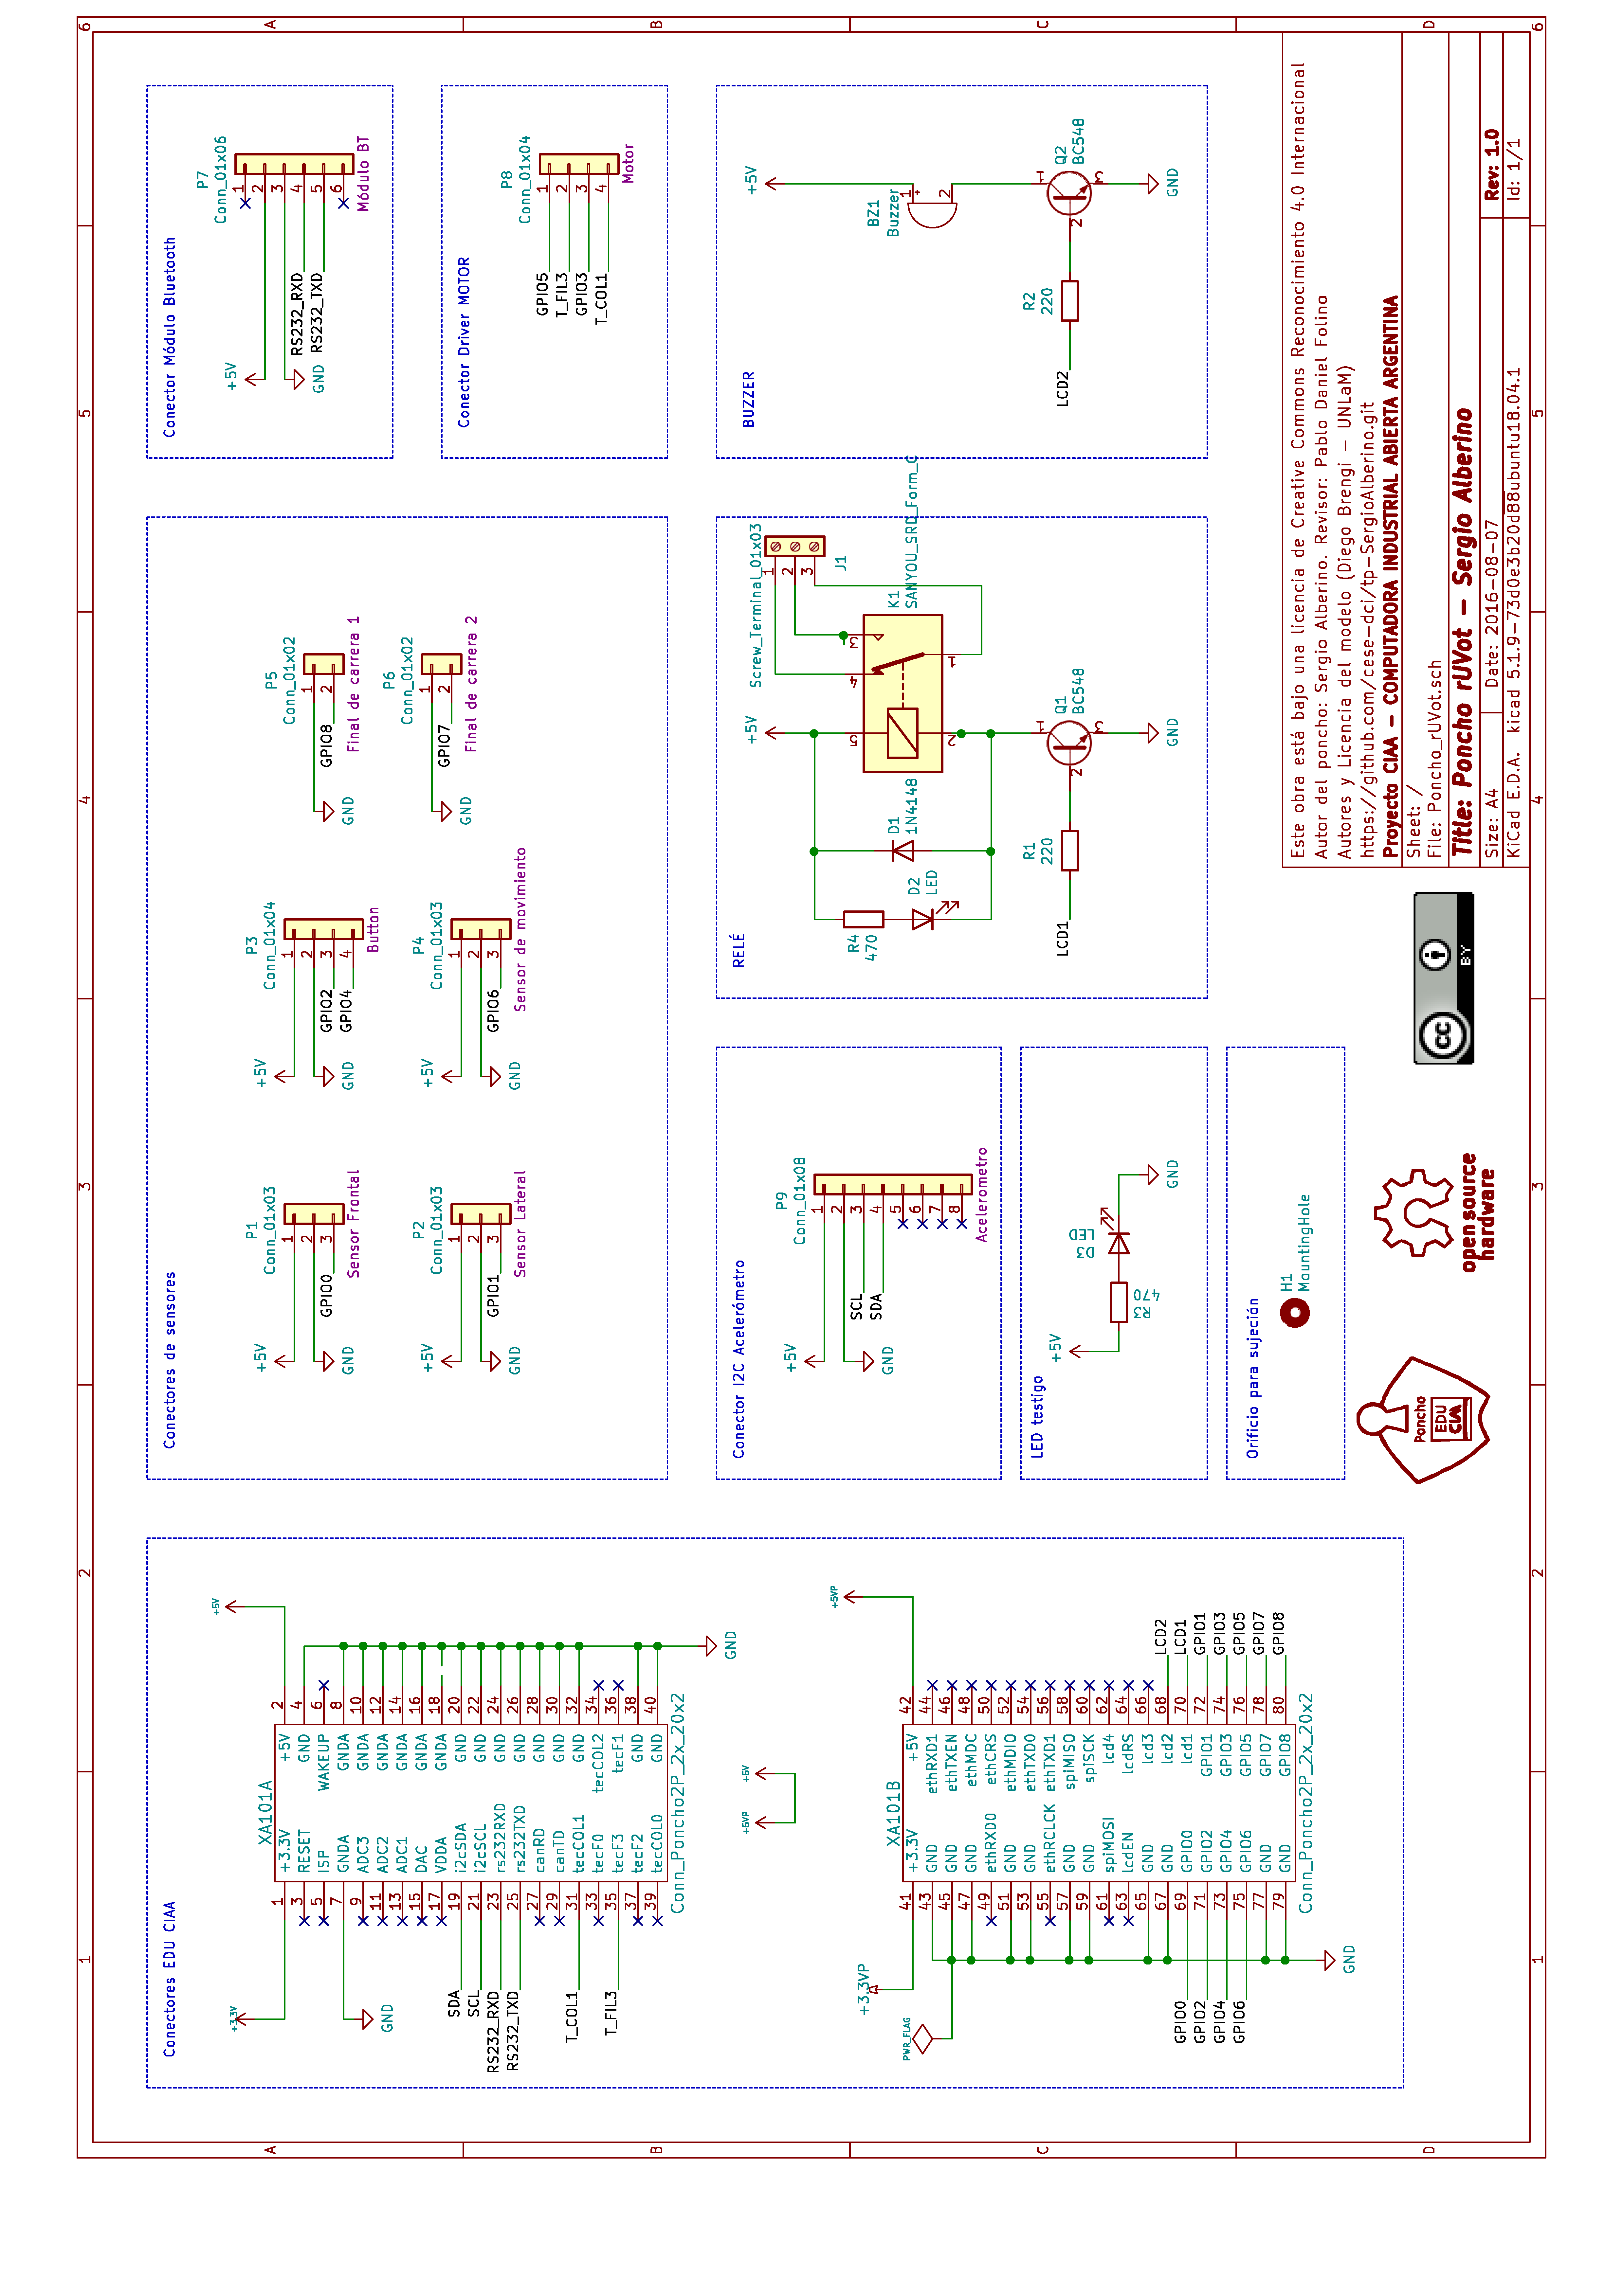
\includegraphics[width=\textwidth]{./Figures/esquematico.png}
%	\caption{Circuito esquemático del poncho.}
%	\label{fig:esquematico}
%\end{figure}
%\pagebreak

%\subsection{Esquema de  de comunicaciones}


%
%
%
%
%\begin{verbatim}
%\begin{lstlisting}[caption= "un epígrafe descriptivo"]
%	las líneas de código irían aquí...
%\end{lstlisting}
%\end{verbatim}
%
%A modo de ejemplo:
%
%\begin{lstlisting}[label=cod:vControl,caption=Pseudocódigo del lazo principal de control.]  % Start your code-block
%
%#define MAX_SENSOR_NUMBER 3
%#define MAX_ALARM_NUMBER  6
%#define MAX_ACTUATOR_NUMBER 6
%
%uint32_t sensorValue[MAX_SENSOR_NUMBER];		
%FunctionalState alarmControl[MAX_ALARM_NUMBER];	//ENABLE or DISABLE
%state_t alarmState[MAX_ALARM_NUMBER];						//ON or OFF
%state_t actuatorState[MAX_ACTUATOR_NUMBER];			//ON or OFF
%
%void vControl() {
%
%	initGlobalVariables();
%	
%	period = 500 ms;
%		
%	while(1) {
%
%		ticks = xTaskGetTickCount();
%		
%		updateSensors();
%		
%		updateAlarms();
%		
%		controlActuators();
%		
%		vTaskDelayUntil(&ticks, period);
%	}
%}
%\end{lstlisting}



